\documentclass[conference]{IEEEtran}
\IEEEoverridecommandlockouts
% ICRA submission. Build from this directory:
%   latexmk -pdf main.tex
% Shared assets live one level up: ../refs.bib and ../images/.
% Constants for the ICRA paper (ICRA/main.tex and ICRA/sections/*.tex).
% Derived from journal/constants.tex; kept separate so the two papers can
% diverge. Macro names keep the \corl prefix so text can move between them.
%
% Convention: every macro holds a bare value (a number, or a short math
% expression like 10^{-3}) with NO unit, %, or $ baked in. Units, percent
% signs, and math-mode delimiters are added at the call site.
%
% Provenance tags:
%   [code]    verified against gait-net source (file noted)
%   [runs]    from gait-net/runs/*/README.md (author records, not re-measured)
%   [comment] from a code comment (author record, not re-measured)
%   [pending] placeholder; fill in once the experiment finishes

% --- Control loop / action timing (training, Isaac Lab) ---
\newcommand{\corlControlHz}{25}            % [code] gaitnet_env_cfg.py: decimation 10
\newcommand{\corlControlTickMs}{40}
\newcommand{\corlPhysicsDtMs}{4}           % [code] gaitnet_env_cfg.py: sim dt 0.004
\newcommand{\corlTrainMpcHz}{50}           % [code] iterations_between_mpc=5 at 250 Hz
\newcommand{\corlSwingDurationMin}{0.1}
\newcommand{\corlSwingDurationMax}{0.3}
\newcommand{\corlMinTicksPerSwing}{3}
\newcommand{\corlMaxTicksPerSwing}{8}
\newcommand{\corlMaxConcurrentSwingLegs}{2}
\newcommand{\corlMinContactLegs}{3}
\newcommand{\corlMaskDilationRounds}{2}
\newcommand{\corlMaskResolutionCm}{1.5}

% --- Tracking state vector (x_t) dimensions ---
\newcommand{\corlStateDim}{25}
\newcommand{\corlFootPosDim}{8}
\newcommand{\corlVelDim}{3}
\newcommand{\corlAngVelDim}{3}
\newcommand{\corlGravityDim}{3}
\newcommand{\corlContactDim}{4}

% --- Network architecture ---
\newcommand{\corlStateEncoderLayers}{3}
\newcommand{\corlStateEncoderHidden}{128}
\newcommand{\corlFootstepEncoderLayers}{2}
\newcommand{\corlFootstepEncoderHidden}{64}
\newcommand{\corlTrunkLayers}{3}

% --- Candidate enumeration and selection (deployment) ---
% Dense = every valid mask cell scored exactly. [comment]
% load_controller.launch:113-117, gaitnetservice.py:405-414.
\newcommand{\corlNumLegs}{4}
\newcommand{\corlGridCells}{25}
\newcommand{\corlGridReachCm}{18}
\newcommand{\corlCellsPerLeg}{625}
\newcommand{\corlSpatialCandidates}{2500}
\newcommand{\corlTotalCandidatesDense}{2501}
\newcommand{\corlDenseScoreMs}{3.68}       % [comment] isolated process
\newcommand{\corlSampledScoreMs}{4.6}      % [comment]
\newcommand{\corlDenseAgreement}{7 \times 10^{-6}}

% --- Training candidate distribution and RL setup ---
\newcommand{\corlTrainCandidatesPerLeg}{16}
\newcommand{\corlTrainTotalCandidates}{65}
\newcommand{\corlDurationExploreStd}{0.01}
\newcommand{\corlActionPenalty}{-0.1}
\newcommand{\corlTerminationPenalty}{-200}
\newcommand{\corlTrainingIterations}{700}
\newcommand{\corlParallelEnvs}{100}

% --- Execution stack (Gazebo and Go1 share legged_perceptive_controllers) ---
\newcommand{\corlNmpcHz}{100}              % [code] go1/task.info mpcDesiredFrequency
\newcommand{\corlNmpcHorizon}{0.8}         % [code] go1/task.info timeHorizon (s)
\newcommand{\corlWbcHz}{500}               % [code] legged_unitree_hw go1.yaml loop_frequency
\newcommand{\corlGazeboStepMs}{1}          % [code] empty_world.world max_step_size
\newcommand{\corlElevMapSizeM}{6}          % [code] elevation_mapping.yaml
\newcommand{\corlElevMapResCm}{4}          % [code] elevation_mapping.yaml

% --- Hardware adapter settings used in the Go1 runs ---
% [code] load_controller.launch at 4d8b6f8 (in effect for the 2026-09-10 runs)
\newcommand{\corlHwRequestPeriod}{0.25}    % s, gates every GaitNet request
\newcommand{\corlHwNoopCooldown}{0.2}      % s
\newcommand{\corlHwMinSwingDuration}{0.25} % s, floor applied to the duration head
\newcommand{\corlHwMaxFootSpeed}{0.8}      % m/s, travel-based duration floor
\newcommand{\corlHwMaxSwingDuration}{0.6}  % s, cap on the floored duration
\newcommand{\corlHwNoopLogitPenalty}{7.0}  % [runs] launch override
\newcommand{\corlHwRepeatPenalty}{1.5}     % [code] hardware default

% --- Gazebo benchmark protocol (TODO: confirm against the final sweep) ---
\newcommand{\corlDifficultyMin}{0}
\newcommand{\corlDifficultyMax}{40}
\newcommand{\corlDifficultyStep}{5}
\newcommand{\corlHighDifficultyRangeLow}{30}
\newcommand{\corlVelocityMin}{0.05}
\newcommand{\corlVelocityMax}{0.2}
\newcommand{\corlSimTrialsPerCell}{XX}     % [pending]
\newcommand{\corlSimEpisodeDuration}{XX}   % [pending]

% --- Gazebo results [pending] ---
\newcommand{\corlGzFullSuccess}{XX}
\newcommand{\corlGzDiagSuccess}{XX}
\newcommand{\corlGzSingleSuccess}{XX}
\newcommand{\corlGzSchedSuccess}{XX}
\newcommand{\corlGzFullSuccessHard}{XX}
\newcommand{\corlGzSchedSuccessHard}{XX}
\newcommand{\corlGzImprovementPts}{XX}
\newcommand{\corlGzOverlapPct}{XX}
\newcommand{\corlGzDenseSuccess}{XX}
\newcommand{\corlGzSampledSuccess}{XX}
\newcommand{\corlGzServiceLatencyMs}{XX}
\newcommand{\corlGzServiceLatencyPNinetyMs}{XX}

% --- Go1 proof-of-concept [runs] (verify against bag [config] lines) ---
\newcommand{\corlHwTerrainBlockMinMm}{40}
\newcommand{\corlHwTerrainBlockMaxMm}{50}
\newcommand{\corlHwTrackLengthM}{1.5}
\newcommand{\corlHwCommandSpeed}{0.05}
\newcommand{\corlHwTerrainAttempts}{7}
\newcommand{\corlHwTerrainSuccesses}{6}
\newcommand{\corlHwOverlapPairs}{13}
\newcommand{\corlHwOverlapMedianMs}{17}
\newcommand{\corlHwOverlapMaxMs}{67}
\newcommand{\corlHwOverlapPct}{0.3}
\newcommand{\corlHwNominalSwingMs}{250}
\newcommand{\corlHwServiceLatencyMinMs}{5}   % [comment] dense-mode service latency
\newcommand{\corlHwServiceLatencyMaxMs}{13}  % [comment]


\usepackage{cite}
\usepackage{amsmath,amssymb,amsfonts}
\usepackage{algorithmic}
\usepackage{graphicx}
\usepackage{textcomp}
\usepackage[table,xcdraw]{xcolor}
\usepackage[colorlinks=true, allcolors=blue]{hyperref}
\usepackage{float}
\usepackage{multirow}
\usepackage{caption}
\usepackage{subcaption}
\usepackage{booktabs}
\usepackage{array}
\usepackage{adjustbox}
\usepackage{fmtcount}

\graphicspath{{../}}

% \pending{...} ORANGE: a number, claim, or figure that depends on
% experiments that have not finished (Gazebo benchmark, extra Go1 trials).
\newcommand{\pending}[1]{\textcolor{orange}{#1}}
% \verify{...} MAGENTA: taken from run logs, READMEs, or code comments;
% confirm against the raw data before submission.
\newcommand{\verify}[1]{\textcolor{magenta}{#1}}

\begin{document}

\title{GaitNet: Controller-Decoupled High-Rate Footstep Selection for
  Acyclic Quadruped Locomotion}

\author{Anonymous Authors}

\maketitle

\begin{abstract}
  Fixed gait schedules decide in advance which leg moves and when.
  This makes locomotion control tractable, but it also restricts
  foothold selection when safe footholds appear at irregular times
  and places. We present GaitNet, a learned planner that makes only
  the discrete contact decision. Every \corlControlTickMs\,ms it
  selects one leg, one foothold, and one swing duration, or it selects
  no action. Swings last several decisions, so the planner can commit
  a new step while another leg is still in the air. Multi-leg
  coordination therefore emerges from repeated single-leg decisions,
  without a gait phase, predefined leg pairs, or a contact schedule.
  Each candidate is scored independently, so a policy trained with
  PPO on sampled candidates in Isaac Lab is deployed, frozen, on an
  exhaustive enumeration of every terrain-valid cell. GaitNet
  communicates with the execution controller through a narrow
  interface and never accesses its internal optimization. We evaluate
  the frozen planner systematically in Gazebo with a
  \texttt{legged\_control} NMPC/WBC execution stack that differs from
  the controller used in training. \pending{Systematic Gazebo
  experiments show that unrestricted GaitNet improves success over
  scheduled and concurrency-restricted alternatives, by
  \corlGzImprovementPts{} percentage points on average, with the
  largest gains at high terrain difficulty.} Limited Unitree Go1
  experiments further demonstrate deployment of the frozen policy
  through the same NMPC/WBC execution stack.
\end{abstract}


\begin{IEEEkeywords}
  Legged Robots, Footstep Planning, Reinforcement Learning
\end{IEEEkeywords}

\section{Introduction}
\label{sec:introduction}

Legged robots can cross broken or narrow terrain as long as a sequence
of usable footholds exists. Finding that sequence requires more than
choosing foothold positions. The robot must also decide which leg
moves, when it lifts off, and how long its swing lasts. We call this
joint discrete decision \textit{contact selection}. We use
\textit{acyclic} for contact sequences that are neither a periodic
gait cycle nor transitions through a fixed gait library; the
literature also uses \textit{non-gaited} and \textit{free-gait}.

Most deployed model-based stacks fix the contact schedule in advance
and optimize motion around it \cite{Kim2019highly-dynamic,
Wensing2022Nov, grandia_perceptive_2022}. This is effective on regular
terrain, but a scheduled leg must step even when no good foothold is
reachable, and an unscheduled leg cannot step even when one is.

GaitNet makes only the contact decision. At each tick it outputs a
leg, a foothold, and a swing duration, or no action. It does
\emph{not} generate joint torques, joint positions, contact forces,
base trajectories, or whole-body control (WBC) objectives. A
downstream model-based controller realizes the decision. This
division keeps the learned component small enough to re-evaluate at a
high rate, and it keeps the foothold explicit so that the controller
can still check it against the terrain before execution.

\subsection{Related Work}
\label{subsec:related-work}

\textit{Optimization and search.} When contacts are decision
variables, planning becomes a mixed-integer program
\cite{Geisert2019contact-planning}. Convex terrain regions
\cite{deits_footstep_2014} and joint optimization of schedule and
timing \cite{winkler_gait_2018, aceituno_simultaneous_2019} shrink the
problem, but remain costly for fast reactive correction. Free-gait and
utility-based planners choose contact timing online from per-leg rules
\cite{fankhauser_free_gait_2016, boussema_online_2019,
bjelonic_whole-body_2021}, and search-based planners generate acyclic
sequences directly \cite{amatucci_monte_2022}. Recent work accelerates
search by learning cost-to-go \cite{taouil_non-gaited_2024} or
transition feasibility \cite{akizhanov_learning_2024}.
Contact-implicit MPC discovers contacts from dynamics in real time
\cite{kim_contact-implicit_2025}, but does not select footholds from a
perceived steppability map.

\textit{Learned controllers and hybrid planners.} End-to-end policies
cross difficult terrain reliably \cite{zhang_learning_2023,
zhang_novel_2024, duan_sim--real_2022, siekmann_blind_2021,
lee_learning_2020}, but the contact decision is implicit in joint
targets and cannot be inspected or constrained before execution.
Hybrid methods learn foothold placement while a gait generator
provides the schedule \cite{gangapurwala_rloc_2022,
villarreal_fast_2019, omar_fast_2022, omar_safesteps_2023,
asselmeier_steppability-informed_2024, gaspard_footstepnet_2024,
tsounis_deepgait_2020, shi_terrain-aware_2023, xie_glide_2023}, or
learn contact structure while a heuristic provides footholds
\cite{da_learning_2020, yang_fast_2021, sun_online_2024}. Patrizi et
al. \cite{patrizi_rl-augmented_2026} learn per-foot flight-phase
injections into an MPC horizon, which yields acyclic timing but not
foothold selection.

\textit{ContactNet.} The closest method is ContactNet
\cite{bratta_contactnet_2024}, which ranks discretized foothold
candidates with a neural network. Its concurrency is set by
configuration: one leg at a time in walking experiments and joint
footholds for a swinging pair in trot experiments. It re-ranks at
touchdown, and the configured gait sets swing timing.
\autoref{tab:capabilities} summarizes the differences we rely on.
Entries for ContactNet reflect only what is reported in
\cite{bratta_contactnet_2024}.

\begin{table}[t]
  \centering
  \caption{Contact-decision capabilities.}
  \label{tab:capabilities}
  \footnotesize
  \setlength{\tabcolsep}{2.5pt}
  \begin{tabular}{lccc}
    \toprule
    \textbf{Capability} & \textbf{Scheduled} & \textbf{ContactNet
    \cite{bratta_contactnet_2024}} & \textbf{GaitNet} \\
    \midrule
    Explicit foothold & Yes & Yes & Yes \\
    Chooses leg & Scheduled & Config.-dependent & Yes \\
    Chooses swing duration & Fixed & No & Yes$^{\dagger}$ \\
    Explicit no-action option & Implicit & \verify{Not reported} & Yes \\
    Re-decides during a swing & No & No (at touchdown) & Yes \\
    Swing overlap & Scheduled & Configured & Emergent \\
    \bottomrule
  \end{tabular}\\[2pt]
  \footnotesize{$^{\dagger}$The Go1 deployment floors the duration
  (\autoref{subsec:exp-hardware}).}
\end{table}

\subsection{Contributions}

\begin{enumerate}
  \item \textbf{High-rate acyclic selection.} A planner that selects
    one leg-specific foothold, swing duration, or no-action every
    \corlControlTickMs\,ms, without representing gait phase,
    predefined leg pairs, or a contact schedule.
  \item \textbf{Set-size-independent scoring.} A per-candidate
    architecture trained with sampled candidates but deployable
    through exhaustive batched enumeration without retraining.
  \item \textbf{Controller-decoupled execution.} A narrow
    planner-controller interface that lets the frozen planner operate
    with a model-based NMPC/WBC execution stack without accessing its
    internal optimization.
  \item \textbf{Systematic evaluation.} Matched Gazebo experiments
    studying terrain difficulty, concurrency restrictions, candidate
    enumeration, timing behavior, and computation, supplemented by a
    proof-of-concept Go1 deployment.
\end{enumerate}

An earlier thesis \cite{Sullivan2025} documented the initial
development of GaitNet. This paper provides its first archival
presentation and systematic evaluation, including exhaustive
deployment-time enumeration, controller transfer, concurrency
ablations, and physical deployment.

\section{Method}
\label{sec:method}

\subsection{System Architecture}
\label{subsec:method-architecture}

GaitNet is the contact-selection layer of a hierarchical stack
(\autoref{fig:architecture}). A terrain map is converted into a
per-leg validity mask. GaitNet scores every valid cell together with a
learned no-action option and issues at most one footstep command. The
execution controller turns that command into a contact schedule, a
swing trajectory, and joint torques. \autoref{tab:stack} lists the
components used at each stage. The same policy weights are used in
all stages; they are frozen after training and are not fine-tuned.

\begin{table}[t]
  \centering
  \caption{Components used at each stage.}
  \label{tab:stack}
  \footnotesize
  \setlength{\tabcolsep}{2.5pt}
  \newcolumntype{L}[1]{>{\raggedright\arraybackslash}p{#1}}
  \begin{tabular}{@{}L{0.17\linewidth}L{0.26\linewidth}L{0.26\linewidth}L{0.26\linewidth}@{}}
    \toprule
    & \textbf{Training} & \textbf{Evaluation} & \textbf{Hardware} \\
    \midrule
    Platform & Isaac Lab \cite{mittal_orbit_2023}, $\Delta t{=}\corlPhysicsDtMs$\,ms
      & Gazebo (ODE), $\Delta t{=}\corlGazeboStepMs$\,ms & Unitree Go1 \\
    Controller & Convex MPC \cite{di_mini_cheetah_2020,
      zhuang_rl_mpc_locomotion_2025}, \corlTrainMpcHz\,Hz
      & NMPC/WBC \cite{leggedcontrol, leggedperceptive}
      & NMPC/WBC \cite{leggedcontrol, leggedperceptive} \\
    NMPC / WBC rate & -- & \corlNmpcHz\,Hz / \verify{XX}\,Hz
      & \corlNmpcHz\,Hz / \corlWbcHz\,Hz \\
    Terrain source & Ray-cast height field & Simulated depth camera
      $\rightarrow$ elevation map & Intel D435i $\rightarrow$
      elevation map \\
    Planner rate & \corlControlHz\,Hz & \pending{\corlControlHz\,Hz}
      & $\le$\,4\,Hz (\autoref{subsec:exp-hardware}) \\
    Policy weights & Trained & Frozen & Frozen \\
    \bottomrule
  \end{tabular}
\end{table}

\begin{figure*}[t]
  \centering
  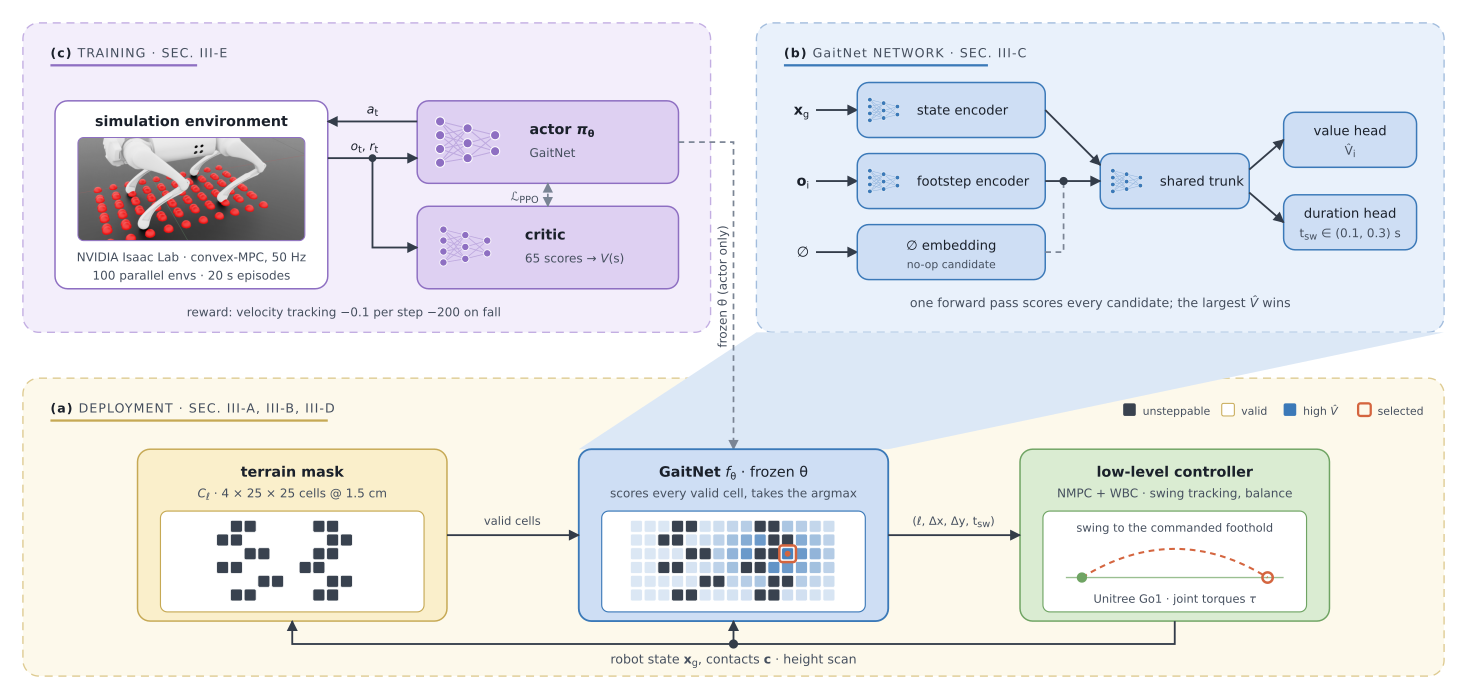
\includegraphics[width=\textwidth]{images/diagrams/gaitnet-architecture.png}
  \caption{System overview. (a)~Deployment: an elevation map becomes a
    per-leg validity mask; GaitNet scores every valid cell plus a
    no-action option in one batched pass, and the argmax is issued as a
    single footstep command to the execution controller. (b)~Network:
    state and candidate embeddings feed a shared trunk with value and
    duration heads. (c)~Training: PPO in Isaac Lab over a sampled
    \corlTrainTotalCandidates-candidate set; only the actor is
    deployed.}
  \label{fig:architecture}
\end{figure*}

In both Gazebo and on the Go1, execution uses the
\texttt{legged\_control} NMPC/WBC framework \cite{leggedcontrol} with
its perceptive extension \cite{leggedperceptive}, built on OCS2. The
NMPC is solved with SQP at \corlNmpcHz\,Hz over a
\corlNmpcHorizon\,s horizon, and a weighted WBC computes joint
torques. The native gait scheduler is replaced by GaitNet commands;
the NMPC, WBC, state estimator, and terrain pipeline are unchanged.
The terrain pipeline builds an elevation map
(\corlElevMapSizeM$\times$\corlElevMapSizeM\,m, \corlElevMapResCm\,cm
cells) from a depth point cloud and decomposes it into convex planar
regions. In Gazebo the point cloud comes from a simulated depth camera,
not from ground-truth geometry, so perception error is present in
evaluation.

\subsection{Planner--Controller Interface}
\label{subsec:method-interface}

At decision time $t$, GaitNet implements the map
\begin{equation}
  \mathcal I_t = \left(x_t,\ \mathcal M_t,\ c_t\right)
  \longmapsto
  \left(\ell_t,\ \Delta p_t,\ T^{\mathrm{swing}}_t\right).
  \label{eq:interface}
\end{equation}
The inputs are:
\begin{itemize}
  \item $x_t$: a controller-independent measured robot state
    (\autoref{eq:state});
  \item $\mathcal M_t = \{M^{i}_t\}_{i=1}^{4}$: per-leg Boolean
    validity masks, each a $\corlGridCells\times\corlGridCells$ grid
    with \corlMaskResolutionCm\,cm cells centered on the projection of
    hip $i$ and aligned with the base yaw;
  \item $c_t\in\{0,1\}^{4}$: per-leg contact/swing status.
\end{itemize}
The outputs are:
\begin{itemize}
  \item $\ell_t \in \{\mathrm{FR},\mathrm{FL},\mathrm{RR},\mathrm{RL},
    \varnothing\}$: the selected leg, where $\varnothing$ denotes no
    action;
  \item $\Delta p_t \in \mathbb R^2$: the foothold target as an $xy$
    offset from the selected hip in the yaw-aligned base frame. The
    target height is taken from the terrain map, not from GaitNet;
  \item $T^{\mathrm{swing}}_t$: the requested swing duration.
\end{itemize}

The controller realizes a command as follows. The foothold is anchored
in the odometry (world) frame at commit time, so it does not drift
with the base during the swing. The swing interval is inserted into
the NMPC mode schedule, and the foothold is passed to the
convex-region selector, which projects it onto the best planar region
and constrains the swing target near the projected point. GaitNet
never reads the NMPC cost, constraints, or solution.

This interface assumes an execution controller that
(i)~accepts explicit foothold targets; (ii)~accepts, or can
approximate, the requested swing duration; (iii)~tracks a commanded
base velocity; (iv)~provides estimated body and foot states; and
(v)~provides contact or swing status. GaitNet is decoupled from the
controller's internal formulation, but it is not independent of
controller tracking quality.

\subsection{High-Rate Acyclic Selection}
\label{subsec:method-selection}

GaitNet is trained to decide every \corlControlTickMs\,ms
(\corlControlHz\,Hz). Each decision issues at most one footstep; all
other legs keep their current commands. Because a swing lasts
\corlSwingDurationMin--\corlSwingDurationMax\,s, between
\numberstringnum{\corlMinTicksPerSwing} and
\numberstringnum{\corlMaxTicksPerSwing} decisions occur before the
swinging leg touches down. At each of them GaitNet may commit another
leg. Swing overlap therefore arises from the value function and the
repeated decision rule, not from a configured gait.

Two feasibility rules are applied before scoring. A leg already in
swing is removed from the mask and its target is not redirected. A new
step is permitted only if at least
\numberstringnum{\corlMinContactLegs} legs are in contact, which
bounds concurrency at \numberstringnum{\corlMaxConcurrentSwingLegs}
swinging legs. In training the mask is additionally dilated with
\numberstringnum{\corlMaskDilationRounds} rounds of max pooling to
account for foot size and state-estimation error.

\subsection{Network}
\label{subsec:method-network}

The robot state is
\begin{equation}
  x_t =
  \begin{bmatrix}
    \mathbf p_{f,xy}^{b} &
    p_{b,z}^{w} &
    \mathbf v_b^{b} &
    \boldsymbol\omega_b^{b} &
    \mathbf v^{\mathrm{cmd}} &
    c_t &
    \mathbf g^{b}
  \end{bmatrix}^\top \in \mathbb R^{\corlStateDim},
  \label{eq:state}
\end{equation}
where superscript $b$ denotes the base frame and $w$ the world
(odometry) frame. $\mathbf p_{f,xy}^{b}\in\mathbb R^{\corlFootPosDim}$
holds the $xy$ positions of the four feet, $p_{b,z}^{w}$ is base
height, $\mathbf v_b^{b}$ and $\boldsymbol\omega_b^{b}$ are base linear
and angular velocity, $\mathbf v^{\mathrm{cmd}}=[v_x,v_y,\omega_z]$ is
the commanded base velocity, and $\mathbf g^{b}$ is the unit gravity
vector expressed in the base frame. Using projected gravity avoids a
quaternion input and its ordering convention.

A \numberstringnum{\corlStateEncoderLayers}-layer MLP (hidden size
\corlStateEncoderHidden) encodes $x_t$. A
\numberstringnum{\corlFootstepEncoderLayers}-layer MLP (hidden size
\corlFootstepEncoderHidden) encodes each candidate's leg one-hot and
hip-relative offset; the no-action option uses a separate learned
embedding. The two embeddings are concatenated
\cite{feng2021deep} and passed through a
\numberstringnum{\corlTrunkLayers}-layer trunk with two heads. The
value head outputs an unnormalized logit $\hat V$ used for ranking,
and the duration head outputs $T^{\mathrm{swing}}$, mapped by a sigmoid
into $(\corlSwingDurationMin,\corlSwingDurationMax)$\,s. All
activations are ReLU.

\subsection{Candidate Enumeration}
\label{subsec:method-enumeration}

At deployment, GaitNet enumerates every mask cell rather than sampling.
Each leg's grid spans $\pm\corlGridReachCm$\,cm around the hip, giving
$\corlNumLegs\times\corlCellsPerLeg=\corlSpatialCandidates$ footholds
plus no-action, i.e.\ \corlTotalCandidatesDense{} candidates. Invalid
cells are discarded before scoring.

Enumeration is cheap because the candidate embedding does not depend
on the state. The embeddings of all grid cells are computed once and
cached, so each decision requires one state-encoder pass and one
batched trunk pass. In an isolated process, scoring all
\corlTotalCandidatesDense{} candidates takes \corlDenseScoreMs\,ms and
agrees with the unfactored forward pass to within
$\corlDenseAgreement$; re-creating the
\corlTrainTotalCandidates-candidate sampled set takes
\corlSampledScoreMs\,ms and can miss the best valid cell. GaitNet
selects the exact argmax of $\hat V$ over all valid cells and
no-action. If no-action wins, or no cell is valid, no step is issued.

The number of candidates is not built into the actor's weights. The
actor is trained on \corlTrainTotalCandidates{} sampled candidates and
deployed on up to \corlTotalCandidatesDense{} without retraining. The
deployed grid is a superset of the training grid, so deployment
changes how many candidates are compared, not what kind of candidate
the network sees.

\subsection{Training}
\label{subsec:method-training}

Labels for optimal contact decisions are not available, because the
value of a step depends on future contacts and body motion. GaitNet is
therefore trained with PPO \cite{Schulman_proximal_2017} in Isaac Lab
with \corlParallelEnvs{} parallel environments of a Go1 model. The
execution controller during training is a Python convex MPC derived
from the MIT Mini-Cheetah controller \cite{di_mini_cheetah_2020,
zhuang_rl_mpc_locomotion_2025}, running at \corlTrainMpcHz\,Hz on CPU.
This is a different controller from the NMPC/WBC stack used in
evaluation.

During training, \numberstringnum{\corlTrainCandidatesPerLeg}
candidates per leg are sampled uniformly from the valid mask and one
no-action option is added, giving \corlTrainTotalCandidates{}
candidates. The actor's logits over this set define a categorical
distribution; sampling keeps its size and entropy bounded. For the
selected candidate, the duration head defines the mean of a Normal
distribution with standard deviation \corlDurationExploreStd\,s, and
the action log-probability is the sum of the categorical and Normal
terms. The critic is a separate network whose per-candidate scores are
combined by a fixed-width MLP into a state value; it is discarded after
training, so the set-size independence applies only to the actor.
Rewards combine velocity tracking, stability, and a per-step action
penalty ($\corlActionPenalty$). Falling or stepping onto invalid terrain
terminates the episode with a $\corlTerminationPenalty$ penalty.
Terrain difficulty follows a curriculum. The policy is trained for
\corlTrainingIterations{} iterations; reward terms and PPO
hyperparameters follow \cite{Sullivan2025}.

\section{Experiments}
\label{sec:experiments}

We ask four questions. (Q1)~Does unrestricted high-rate contact
selection improve success as terrain becomes harder? (Q2)~How much of
the benefit comes from emergent concurrency? (Q3)~Does exhaustive
enumeration matter relative to sampling? (Q4)~Can the frozen planner
run in real time with a model-based stack on a physical robot?

\subsection{Training and Deployment Setup}
\label{subsec:exp-setup}

All conditions use one PPO checkpoint trained as in
\autoref{subsec:method-training}, frozen after training. Conditions
differ only in the action-selection constraints listed below, applied
to the same logits. \pending{Random seeds, the checkpoint hash, and all
launch parameters are logged for every trial.}

\subsection{Gazebo Terrain Benchmark}
\label{subsec:exp-gazebo}

\textit{Terrain.} Each world is a grid of rigid tiles on pillars with
a fraction of tiles removed; removed tiles are true drops rather than
painted regions. Terrain difficulty is the percentage of removed tile
area, from $\corlDifficultyMin\%$ to $\corlDifficultyMax\%$ in
$\corlDifficultyStep\%$ steps. \pending{Tile size, track length, and
the world seeds per difficulty level will be reported here.}

\textit{Protocol.} Commanded forward speed ranges from
$\corlVelocityMin$ to $\corlVelocityMax$\,m/s. Each (method,
difficulty, speed) cell is run for \pending{\corlSimTrialsPerCell}
trials of \pending{\corlSimEpisodeDuration}\,s on matched worlds and
seeds. A trial succeeds if the robot reaches the end of the track
without the base contacting the ground, the controller safety check
triggering, or the base height falling below a fixed threshold.

\textit{Conditions.}
\begin{enumerate}
  \item \textbf{Scheduled NMPC:} the native periodic gait of the
    execution stack with its heuristic foothold projected onto convex
    terrain regions \cite{leggedperceptive}.
  \item \textbf{GaitNet-RoundRobin:} GaitNet footholds and durations,
    but legs are served in a fixed cyclic order.
  \item \textbf{GaitNet-Single:} at most one swinging leg. This matches
    the concurrency of ContactNet's walking configuration
    \cite{bratta_contactnet_2024}; ContactNet has no public
    implementation, so we do not compare against it directly.
  \item \textbf{GaitNet-Diagonal:} a second swing is allowed only for
    the diagonal partner of the leg in the air, a trot-like
    restriction.
  \item \textbf{GaitNet-Full:} the proposed planner, with up to
    \numberstringnum{\corlMaxConcurrentSwingLegs} swinging legs and no
    restriction on which legs overlap.
\end{enumerate}

\begin{table}[t]
  \centering
  \caption{Gazebo success rate, mean over speeds.}
  \label{tab:gazebo}
  \small
  \begin{tabular}{lcc}
    \toprule
    \textbf{Method} & \textbf{All difficulties} &
    \textbf{$\ge\corlHighDifficultyRangeLow\%$} \\
    \midrule
    Scheduled NMPC \cite{leggedperceptive} &
      \pending{\corlGzSchedSuccess\%} & \pending{\corlGzSchedSuccessHard\%} \\
    GaitNet-RoundRobin & \pending{XX\%} & \pending{XX\%} \\
    GaitNet-Single & \pending{\corlGzSingleSuccess\%} & \pending{XX\%} \\
    GaitNet-Diagonal & \pending{\corlGzDiagSuccess\%} & \pending{XX\%} \\
    \textbf{GaitNet-Full} & \pending{\textbf{\corlGzFullSuccess\%}} &
      \pending{\textbf{\corlGzFullSuccessHard\%}} \\
    \bottomrule
  \end{tabular}
\end{table}

\begin{figure}[t]
  \centering
  \pending{%
  \setlength{\fboxsep}{0pt}%
  \fbox{\begin{minipage}[c][0.55\linewidth][c]{0.95\linewidth}
    \centering
    \textit{Success rate vs.\ terrain difficulty (pending)}
  \end{minipage}}%
  }
  \caption{Gazebo success rate versus terrain difficulty for all
    conditions, with 95\% Wilson intervals.}
  \label{fig:gazebo-difficulty}
\end{figure}

\pending{\autoref{tab:gazebo} and \autoref{fig:gazebo-difficulty}
report the results. Describe the ordering of methods, where the gap
opens as difficulty increases, and whether differences are
statistically significant (report the test used).}

\subsection{Concurrency Ablation}
\label{subsec:exp-concurrency}

GaitNet-Single, GaitNet-Diagonal, and GaitNet-Full share the same
weights and differ only in which second swing is admissible, so their
difference isolates the contribution of emergent overlap (Q2). We
report the fraction of time with two legs in swing, the distribution
of overlapping leg pairs, and the number of step requests blocked by
the restriction. \pending{In GaitNet-Full, two legs are in swing
\corlGzOverlapPct\% of the time. Report the pair distribution and
whether same-side pairs occur.} An example swing schedule is shown in
\autoref{fig:swing-schedule}.

\begin{figure}[t]
  \centering
  \pending{%
  \setlength{\fboxsep}{0pt}%
  \fbox{\begin{minipage}[c][0.45\linewidth][c]{0.95\linewidth}
    \centering
    \textit{Gazebo swing schedule (pending)}
  \end{minipage}}%
  }
  \caption{Swing schedule from a GaitNet-Full Gazebo trial. Each row
    is one leg; bars are swings.}
  \label{fig:swing-schedule}
\end{figure}

\subsection{Candidate-Enumeration Study}
\label{subsec:exp-enumeration}

To separate the benefit of dense selection from that of the learned
value function (Q3), we evaluate GaitNet-Full with (i)~exhaustive
enumeration of all valid cells and (ii)~the
\corlTrainTotalCandidates-candidate sampled set used in training, and
\pending{(iii)~intermediate per-leg sample counts}. The weights are
identical across settings. \pending{Dense enumeration reaches
\corlGzDenseSuccess\% success versus \corlGzSampledSuccess\% with
sampling.}

\subsection{Computation and Real-Time Feasibility}
\label{subsec:exp-compute}

We measure (i)~the network forward time, (ii)~the end-to-end service
latency from request to response, and (iii)~the realized decision
interval, which also includes request gating in the controller. In an
isolated process, dense scoring takes \corlDenseScoreMs\,ms.
\pending{In Gazebo, the end-to-end service latency is
\corlGzServiceLatencyMs\,ms (p90 \corlGzServiceLatencyPNinetyMs\,ms),
and the realized decision interval is XX\,ms against the
\corlControlTickMs\,ms target.} The NMPC and WBC run at the rates in
\autoref{tab:stack} regardless of planner latency, since the planner
only updates the mode schedule and foothold targets.

\subsection{Physical-Robot Proof-of-Concept}
\label{subsec:exp-hardware}

We deploy the frozen policy on a Unitree Go1 through the same NMPC/WBC
stack (\autoref{tab:stack}), with an Intel RealSense D435i providing
the point cloud. The track is \verify{\corlHwTerrainBlockMinMm--%
\corlHwTerrainBlockMaxMm\,mm blocks on a mat}, the robot is commanded
\verify{\corlHwTrackLengthM\,m at \corlHwCommandSpeed\,m/s}, and a trial
succeeds if the robot reaches the target distance.

\textit{Deployment adaptations.} The hardware run differs from the
Gazebo configuration in ways that we report explicitly:
\begin{itemize}
  \item Requests are gated to at most one every
    \corlHwRequestPeriod\,s, with a \corlHwNoopCooldown\,s cooldown after
    a no-action response, so the realized decision rate is at most
    4\,Hz rather than \corlControlHz\,Hz.
  \item The requested duration is floored at
    $\max(\corlHwMinSwingDuration,\, d/\corlHwMaxFootSpeed)$\,s, where
    $d$ is the swing travel in meters, and capped at
    \corlHwMaxSwingDuration\,s, because the shortest learned swings
    exceed the Go1's achievable foot speed.
  \item A second swing is restricted to the diagonal partner.
  \item The no-action logit is reduced by \corlHwNoopLogitPenalty{}
    and recently used legs receive a penalty of
    \corlHwRepeatPenalty{}.
\end{itemize}
The policy weights are unchanged; these adaptations act on the
interface, not on the network.

\textit{Results.} \verify{GaitNet completed
\corlHwTerrainSuccesses/\corlHwTerrainAttempts{} attempts on the
block track. The single failure was a step that landed short onto a
block.} \verify{In a trial with diagonal overlap enabled, two legs
were simultaneously in swing \corlHwOverlapPct\% of the time
(\corlHwOverlapPairs{} overlapping pairs, all diagonal; median overlap
\corlHwOverlapMedianMs\,ms, maximum \corlHwOverlapMaxMs\,ms, against
\corlHwNominalSwingMs\,ms swings).} Dense-mode service latency was
\verify{\corlHwServiceLatencyMinMs--\corlHwServiceLatencyMaxMs\,ms}.
\pending{Report the planner latency distribution and mean traversal
time if additional trials are collected.} With $n=\corlHwTerrainAttempts$
we make no statistical comparison against any baseline; these trials
establish only that the frozen policy and interface execute on
physical hardware.

\subsection{Limitations}
\label{subsec:exp-limitations}

\textit{Decision rate on hardware.} The high-rate mechanism evaluated
in Gazebo was not reproduced on the Go1, where request gating limited
decisions to at most 4\,Hz and overlap was brief. The hardware trials
therefore demonstrate feasibility of the interface, not the benefit of
high-rate selection.

\textit{Interface adaptations.} The duration floor, diagonal
restriction, and logit penalties are hand-tuned for the Go1. They
reduce the degrees of freedom that GaitNet exercises on hardware, and
their individual effects have not been ablated.

\textit{Controller dependence.} The planner does not access the
controller's internal optimization, but its success depends on the
controller tracking the requested footholds and durations; we have
evaluated one training controller and one execution stack.

\textit{Concurrency bound.} The rule that
\numberstringnum{\corlMinContactLegs} legs remain in contact is fixed
in all experiments and has not been ablated.

\textit{Perception.} The validity mask is thresholded from a planar
decomposition of the elevation map. Small voids below the camera's
effective resolution are not represented, and the sim-to-real gap in
the mask has not been quantified.

\section{Conclusion}
\label{sec:conclusion}

We presented GaitNet, a planner that makes only the discrete contact
decision for a quadruped: one leg, one foothold, and one swing
duration, or no action, re-evaluated while other legs are still in
swing. Because candidates are scored independently, a policy trained
on sampled candidates is deployed without retraining on an exhaustive
enumeration, and its argmax is realized by a model-based NMPC/WBC
stack through a narrow interface.

\pending{Systematic Gazebo experiments demonstrate the benefit of
high-rate unrestricted contact selection.} Limited Go1 experiments
establish that the frozen policy and planner-controller interface can
execute on physical hardware, while larger hardware comparisons remain
future work. Further work will remove the hand-tuned hardware
adaptations by training with the execution controller's timing limits,
restore the trained decision rate on hardware, and learn directly from
elevation maps rather than thresholded masks.


\bibliographystyle{ieeetr}
\bibliography{../refs}

\end{document}
